% =========================================================================
% AAT — Figure: Sector Condition and Error-Space Contraction
% Companion to: #result-sector-condition-stability, #deriv-sector-condition,
%               #disc-stability-certificate
%
% Build:  pdflatex sector-cone.tex
% =========================================================================
\documentclass[border=8pt]{standalone}
\usepackage{tikz}
\usepackage{amsmath,amssymb}
\usetikzlibrary{arrows.meta,calc,decorations.markings,backgrounds,positioning}

\begin{document}
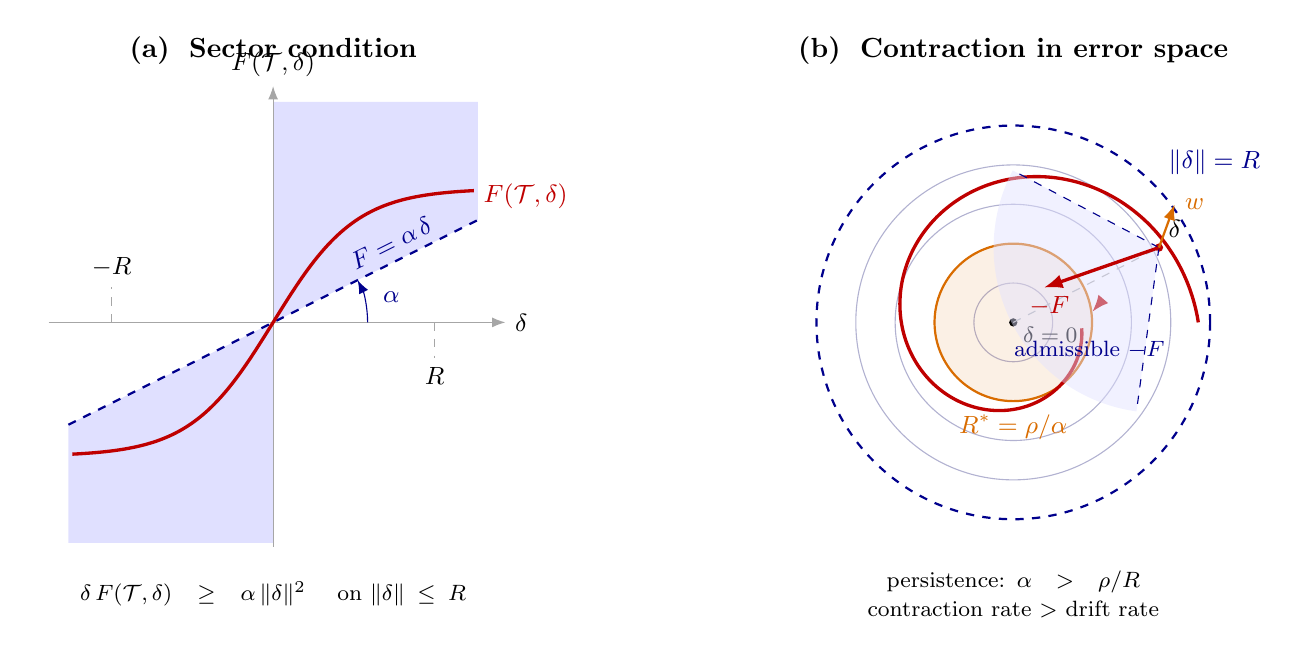
\begin{tikzpicture}[
    font=\small,
    >=Latex,
    contour/.style       = {blue!40!black, opacity=0.30, thin},
    sector-fill/.style   = {blue!12},
    sector-edge/.style   = {blue!55!black, dashed, thick},
    correction/.style    = {red!75!black, very thick, -{Latex[length=2.4mm]}},
    trajectory/.style    = {red!75!black, very thick},
    disturbance/.style   = {orange!85!black, thick, -{Latex[length=2mm]}},
    valid/.style         = {blue!55!black, dashed, thick},
    ultimate/.style      = {orange!85!black, thick}
  ]

% =========================================================
% PANEL (a) — Sector condition in the (delta, F) plane
% =========================================================
\begin{scope}
  % Sector regions: { (delta,F) : delta * F >= alpha * delta^2 }
  % with alpha = 0.5. Two diagonally opposite pieces (Q1 above the line,
  % Q3 below the line), bounded by F = alpha * delta.
  \fill[sector-fill] (0,0) -- (2.6, 1.30) -- (2.6, 2.8) -- (0, 2.8) -- cycle;
  \fill[sector-fill] (0,0) -- (-2.6,-1.30) -- (-2.6,-2.8) -- (0,-2.8) -- cycle;

  % Axes
  \draw[->, gray!70] (-2.85, 0) -- (2.95, 0) node[right, black]{$\delta$};
  \draw[->, gray!70] (0,-2.85) -- (0, 3.00) node[above, black]{$F(\mathcal{T},\delta)$};

  % Sector boundary line F = alpha*delta (slope alpha = 0.5)
  \draw[sector-edge] (-2.6,-1.30) -- (2.6, 1.30);
  \node[blue!55!black, anchor=south, rotate=26.57] at (1.6, 0.80) {$F = \alpha\,\delta$};

  % Example correction function: saturating, leaves sector for |delta| > R
  % F(delta) = 1.7 * tanh(0.95 * delta) ; intersects F=0.5*delta near |delta| ~ 2.05
  \draw[trajectory, smooth, samples=160, domain=-2.55:2.55]
    plot (\x, {1.7*tanh(0.95*\x)});
  \node[red!75!black, anchor=west] at (2.55, 1.60) {$F(\mathcal{T},\delta)$};

  % R markers (where curve exits the sector)
  \draw[dashed, gray!70] (2.05, 0) -- (2.05, -0.45) node[below, black]{$R$};
  \draw[dashed, gray!70] (-2.05, 0) -- (-2.05, 0.45) node[above, black]{$-R$};

  % alpha angle annotation
  \draw[->, blue!55!black, thin] (1.20, 0.0) arc[start angle=0, end angle=26.57, radius=1.20];
  \node[blue!55!black] at (1.50, 0.32) {$\alpha$};

  % Title & caption
  \node[font=\bfseries] at (0, 3.45) {(a)\; Sector condition};
  \node[font=\footnotesize, align=center, text width=6cm] at (0,-3.45)
    {$\delta\,F(\mathcal{T},\delta) \;\geq\; \alpha\,\lVert\delta\rVert^{2}$ \quad on $\lVert\delta\rVert\leq R$};
\end{scope}

% =========================================================
% PANEL (b) — Error-space contraction with ultimate bound
% =========================================================
\begin{scope}[xshift=9.4cm]

  % Lyapunov sublevel sets (concentric circles, V = 1/2 |delta|^2)
  \foreach \r in {0.5, 1.0, 1.5, 2.0} {\draw[contour] (0,0) circle (\r);}

  % Valid region boundary (R) -- where the sector condition holds
  \draw[valid] (0,0) circle (2.5);
  \node[blue!55!black, anchor=south west] at (1.85, 1.75) {$\lVert\delta\rVert = R$};

  % Ultimate-bound ball R* = rho / alpha (trajectories enter and stay)
  \fill[orange!85!black, opacity=0.10] (0,0) circle (1.0);
  \draw[ultimate] (0,0) circle (1.0);
  \node[orange!85!black, anchor=north] at (0,-1.05) {$R^{\ast} = \rho/\alpha$};

  % Equilibrium
  \fill[black] (0,0) circle (1.5pt);
  \node[below right=-2pt and 0pt, font=\footnotesize] at (0,0) {$\delta = 0$};

  % Spiraling trajectory entering R*
  \draw[trajectory, smooth, samples=180, domain=0:6.2]
    plot ({2.35*exp(-0.16*\x)*cos(\x r)}, {2.35*exp(-0.16*\x)*sin(\x r)});
  % Arrowhead on the trajectory
  \draw[trajectory, -{Latex[length=2.2mm]}] (1.06, 0.20) -- (1.00, 0.13);

  % Error point delta on the trajectory
  \coordinate (E) at (1.85, 0.95);
  \fill[red!75!black] (E) circle (1.5pt);
  \node[anchor=south west] at (E) {$\delta$};

  % Radial reference (origin -> delta)
  \draw[gray!60, dashed] (0,0) -- (E);

  % Half-plane / cone of admissible -F directions at delta
  \pgfmathsetmacro{\thetaE}{atan2(0.95, 1.85)} % angle of delta from origin
  \pgfmathsetmacro{\phi}{\thetaE + 180}        % inward radial direction
  \begin{scope}[shift=(E)]
    \fill[sector-fill, opacity=0.45]
      (0,0)
      -- ({2.1*cos(\phi - 55)}, {2.1*sin(\phi - 55)})
      arc[start angle={\phi - 55}, end angle={\phi + 55}, radius=2.1]
      -- cycle;
    \draw[sector-edge, thin]
      (0,0) -- ({2.1*cos(\phi - 55)}, {2.1*sin(\phi - 55)});
    \draw[sector-edge, thin]
      (0,0) -- ({2.1*cos(\phi + 55)}, {2.1*sin(\phi + 55)});
    \node[blue!55!black, font=\footnotesize, anchor=south east]
      at ({1.55*cos(\phi + 70)}, {1.55*sin(\phi + 70)}) {admissible $-F$};
  \end{scope}

  % Actual -F vector (lies inside the wedge)
  \draw[correction] (E) -- ($(E) + ({-1.55*cos(\thetaE - 8)}, {-1.55*sin(\thetaE - 8)})$)
    node[red!75!black, anchor=north, pos=0.95] {$-F$};

  % Disturbance vector w (smaller, pushing outward)
  \draw[disturbance] (E) -- ($(E) + (0.20, 0.55)$)
    node[orange!85!black, anchor=west] {$w$};

  % Title & caption
  \node[font=\bfseries] at (0, 3.45) {(b)\; Contraction in error space};
  \node[font=\footnotesize, align=center, text width=6.4cm] at (0,-3.45)
    {persistence: $\alpha > \rho/R$\\[1pt]
     contraction rate $>$ drift rate};
\end{scope}

\end{tikzpicture}
\end{document}
